
\chapter{Background}
This chapter describes theoretic results that this thesis is based
on. It covers trajectory data, motion pattern learning, supervised machine learning from a
Bayesian perspective, GPs, and arrival time prediction using machine learning.

\section{Trajectory Data}\label{sec:trajectory-data}
A \textit{trajectory} $\traj_{k}$ of can be seen as an ordered collection of
observations $(\obs^{(k)}_1, \obs^{(k)}_2, \dots, \obs^{(k)}_N)$.
The thesis project focuses on \textit{spatio-temporal}
trajectories, which mean that each observation in a trajectory has a position both in time
and in space. A trajectory has a \textit{length} and
a \textit{duration}. The length $\len(\traj_{k}) = N$ is the number of
observations, and the duration $\dur(\traj_{k}) = \text{time}(\obs^{(k)}_N) - \text{time}(\obs^{(k)}_1)$
is the time from the first observation to the last.
These properties are in general not the same for different
trajectories, which makes it hard to compare them in a
meaningful way. Having different lengths makes a comparison
particularly difficult. If a set of trajectories all have the same length, they could
be viewed as vectors, with one observation per dimension, and compared
using Euclidian distance. But trajectories of different lengths do not
exist in the same vector space, so Euclidian distance fails and more
advanced similarity metrics have to be used.
An illustration of trajectories with different length can be seen in Figure~\ref{fig:trajectory-projection-problems}.
\begin{figure}
  \centering
  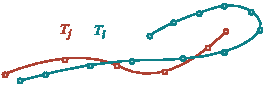
\includegraphics[width=0.7\textwidth]{figures/trajectory-projection-problems}
  \caption{An illustration of two trajectories $\traj_{i}$ and $\traj_{j}$
    with different lengths and duration. There is no natural way of
    measuring the distance between them.}\label{fig:trajectory-projection-problems}
\end{figure}

Even trajectories generated from the same underlying process do not in general
have the same length and duration, even though they are typically more
similar. For instance, a bus driving the same route several times
would not produce trajectories with identical duration and length. 
If two trajectories from the same underlying
process have the same amount of observations at the same time points,
they are said to be \textit{synchronised}. 
Otherwise they are said to be\textit{unsynchronised}.

\section{Supervised Machine Learning}
Supervised machine learning is the process of training computers programs to
recognise patterns in data~\cite{Bishop-2006}. It is incredibly
flexible, and can find patterns such as ``What
temperature is expected for this time of year on this geographical
position?'' or ``What subject is this text about?''. Finding the first
type of pattern of continuous temperature is called
\textit{regression}, and finding the
second pattern with a discrete number of subjects is called
\textit{classification}. Both types of problems have two inputs: 
the \textit{observations}
\[X =
  \begin{pmatrix}
    \obs_{1}^{1} & \obs_{2}^{1} & \cdots & \obs_{D}^{1} \\
    \obs_{1}^{2} & \obs_{2}^{2} & \cdots & \obs_{D}^{2} \\
    \vdots  & \vdots  & \ddots & \vdots  \\
    \obs_{1}^{N} & \obs_{2}^{N} & \cdots & \obs_{D}^{N} \\
  \end{pmatrix},
\]
containing $N$ observations, and the \textit{target vector} $Y = (y_{1},
y_{2}, \dots, y_{N})$. In the first example of predicting temperatures,
$X$ could contain rows of latitude, longitude and time of year, and $Y$ the
corresponding recorded temperatures. The
goal is to learn how the input and output is related by finding a model which approximates a $D$-ary function $y_n =
f(\obs_n)$ for $1 \leq n \leq N$. Such a model could then
predict $y$ for a previously unseen input $\hat{\obs}$. The way a
model approximates $f$ depends entirely on the model, of which there
are many. Common for all models however, is that they are all \textit{trained}
on data. It is during this process they learn the patterns in the data
which they then use to make predictions.
While there are many approaches to this, the remainder of this
section describes the process of selecting and training models,
and using them to make predictions from a Bayesian point of view.

\subsection{Model Training}
The first step is to pick a model for the data, which in a Bayesian
framework is a probability distribution $\prob(\obs \vert \hyperparam)$, where
$\hyperparam$ is a hyper-parameter vector to the distribution. The
probability of all observations is then $\prob(X \vert \hyperparam) =
\prob(\obs_1, \obs_2, \dots, \obs_N \vert \hyperparam)$. For
mathematical convenience it is often assumed that the observed data
come from the same distribution and that each observation is
independent of all other. This means that the probability of a pair of observations $\obs_i$, $\obs_j$ is $\prob(x_i, x_j
\vert \hyperparam) = \prob(\obs_i \vert \hyperparam)\prob(\obs_j
\vert \hyperparam)$ and consequently, that the probability of observing all the data
is $\prob(X \vert \hyperparam) = \prod_{i=1}^N\prob(\obs_i \vert \hyperparam)$.
This is known as the \textit{likelihood}, which describes how likely
the data is given a certain $\hyperparam$. One way of training a model is
by finding $\hat{\hyperparam} = \underset{\hyperparam}{\mathrm{argmax}}$ $\prob(X \vert \hyperparam)$, 
which is called \textit{maximum likelihood}-estimation (ML-estimation), since it picks the
$\hyperparam$ that maximises the likelihood of the data. However, this picks a single
``best value'', highly sensitive to the choice of training data, which
can lead to a problem called \textit{over-fitting}.

\begin{figure}
  \begin{minipage}{.46\textwidth}
    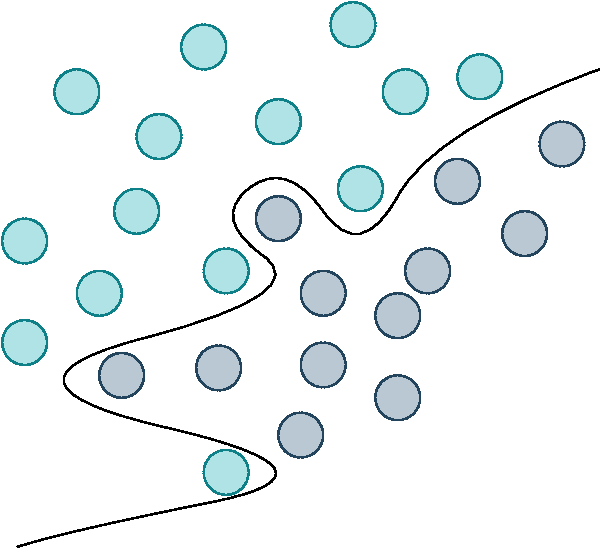
\includegraphics[scale=0.5,width=\textwidth]{figures/over-fit-example}
    \caption{Example of an over-fit in a classification problem. The
      function separating the two classes is too flexible, and captures observations
      which should be consider noise. This model will not generalise well. }\label{fig:over-fit-example}
  \end{minipage}
  \hspace{5pt}
  \begin{minipage}{.46\textwidth}
    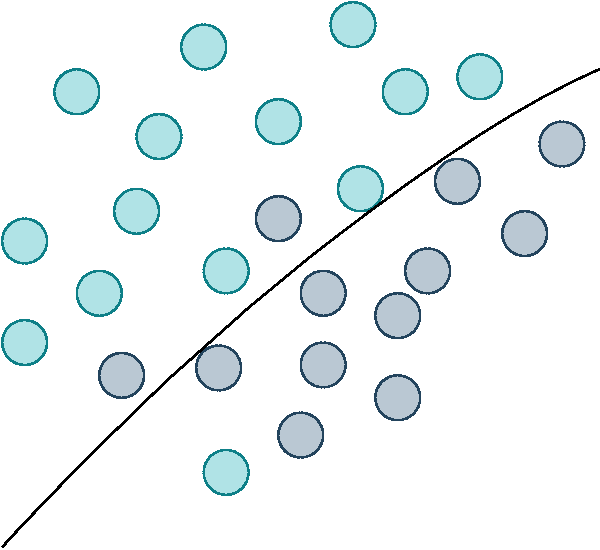
\includegraphics[scale=0.48,width=\textwidth]{figures/good-fit-example}
    \caption{Example of a good fit in a classification problem. The
      function separating the two classes captures the generale structure of the
      data. Even though this misclassifies some observations, this
      model stands a much better chance at generalising.}\label{fig:good-fit-example}
  \end{minipage}
\end{figure}

The goal when training a model is to learn patterns that
\textit{generalise} to unseen data. If $\hyperparam$ is estimated
from data using ML-estimation, it is possible to find a $\hat{\hyperparam}$ that
makes for an increadibly flexible model which \textit{perfectly}
captures the patterns in the data. However, it is very common for data
to contain noise and outliers, which do not represent a pattern that
generalise well. A model that learns these is said to have
\textit{over-fit}, which is highly undesireable. An illustration of
this can be seen in Figure~\ref{fig:over-fit-example}, together with Figure~\ref{fig:good-fit-example}.

One way of avoiding over-fitting is to use \textit{Bayesian inference}, in which 
Bayes theorem
\begin{equation}
  \label{eq:bayes}
  \prob(\hyperparam \vert X) = \frac{\prob(X \vert \hyperparam) \prob(\hyperparam)}{\prob(X)}
\end{equation}
is used to estimate $\hyperparam$ from the \textit{posterior} distribution $\prob(\hyperparam \vert X)$.
This process is called \textit{maximum a posteriori}-estimation (MAP-estimation). To use Bayes
rule a \textit{prior} distribution $\prob(\hyperparam)$ is required, which formalises
a prior belief about $\hyperparam$ before observing any data. The prior is
subjective, and different people may pick different priors,
representing their personal belief about the data. By picking a
prior corresponding to a not-too-flexible model, over-fitting can be
avoided. In the case of GPs, this corresponds to a distribution over kernel
parameter $\hyperparam$ which gives a very wide
kernel. This implies a high correlation between observations further
apart, which in turn implies a slowly-varying function.
In summary, the process of training a model is equivalent to computing
the posterior, from which the most probable model parameters can be
extracted. Training a model using ML- or MAP-estimation both require that the
likelihood can be optimised. This is not always possible to do in
closed form, in which case iterative methods, such as Stochastic
Gradient Descent (SGD) can be used. These types of methods are
prone to to finding local optimas, so random restarts need to be used
to increase the chances of finding a good parametrisation.

If a prior is specified, it is possible to estimate the parameters of
model $\model$ \textit{without} fitting it to data, avoiding the
problem of over-fitting entirely. This is done by maximising the
\textit{marginal likelihood}
\begin{equation}
  \label{eq:marginal-likelihod}
  \prob(\obs \vert \model) = \int \prob(\obs \vert \hyperparam,
  \model) \prob(\hyperparam \vert \model) \prob(\hyperparam) d\hyperparam
\end{equation}
which considers both the uncertainty in $\obs$ and
$\hyperparam$. However, the marginal likelihood is very sensitive to
the choice of prior, so if the prior is not selected carefully this
way of estimating $\hyperparam$ will produce a bad model. The integral
can also be intractable to compute.

\subsection{Making Predictions}
When the model is trained, it can be used to make predictions
about new observations, via the \textit{posterior
  predictive distribution}
\begin{equation}
  \label{eq:posterior-predictive}
  \prob(y \vert X) = \int \prob(y|X,\hyperparam)\prob(\hyperparam \vert X) d \hyperparam,
\end{equation}
\begin{figure}
  \begin{minipage}{.46\textwidth}
    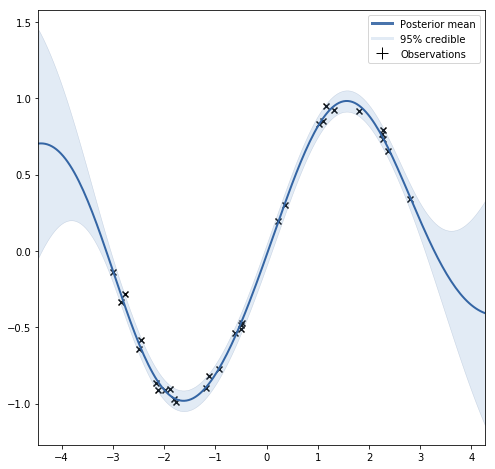
\includegraphics[scale=0.48,width=\textwidth]{figures/high-confidence}
    \caption{Illustration of the 95\% credible intervals for the
    posterior predictive distribution for a regression model. The 
    predictive distribution is narrow, giving tighter
    confidence bands.}\label{fig:high-confidence}
  \end{minipage}
  \hspace{5pt}
  \begin{minipage}{.46\textwidth}
    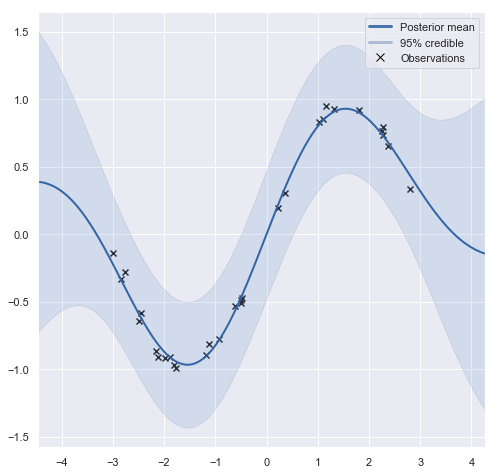
\includegraphics[scale=0.5,width=\textwidth]{figures/low-confidence}
    \caption{Illustration of the 95\% credible intervals for the
    posterior predictive distribution for a regression model. In this
    case the predictive distribution is very wide, giving wider
    confidence bands.}\label{fig:low-confidence}
  \end{minipage}
\end{figure}

which accounts for the parameter uncertainty through the
marginalisation of $\hyperparam$. From the predictive distribution,
very sophisticated predictions can be made. The ``best guess'' of $y$
is represented by $\text{E}[y \vert X]$, and thanks to having
an entire distribution it is possible to compute exactly how certain
it is. This can be done by computing the \textit{credible
  intervals}~\cite{Morey2016Feb} for the distribution, which is the
span in which a certain amount of probability mass lies. For instance,
the 95\%-credible interval would contain 95\% of the probability mass,
which can be interpreted as a 95\% chance of future observations
falling inside this span. An illustration of credible intervals can be seen in
Figure~\ref{fig:high-confidence} and Figure~\ref{fig:low-confidence}.

\section{Arrival Time Prediction}
Arrival time prediction is, in a nutshell, the problem of answering
the question ``When does the bus arrive?''. When viewed as a machine
learning problem, the goal is to
learn a function $\arrtime = f(\obs)$ for arrival time $\arrtime$ and 
state vector $\obs$, which
contains information on the current state of the world. For instance, it
could contain the position of a bus and the time of day.

\subsection{Prediction Evaluation}
The \textit{Mean Absolute Error} (MAE), defined as
\begin{equation}
  \label{eq:mae}
  MAE(\hat{t}, t) = \frac{1}{n}\sum_{i=1}^{n}{\vert \hat{t} - t \vert},
\end{equation}
for true value $\hat{t}$, provides a natural interpretation as 
``the average of the total error'' which is a relevant
and easy-to-understand quantity~\cite{willmott2005advantages}.

%% Two complementary ways of evaluating how good a prediction is are the metrics
%%  (MAE) and \textit{Mean Absolute Percentage
%%   Error} (MAPE), defined for the true value $\hat{t}$ as
%% and
%% \begin{equation}
%%   \label{eq:mape}
%%   MAPE(\hat{t}, t) = \frac{1}{n}\sum_{i=1}^{n} \vert \frac{\hat{t} - t}{\hat{t}} \vert
%% \end{equation}
%% respectively. 

%%  MAPE on the other hand calculates a relative
%% error~\cite{Armstrong1992Jun}, which is unaffected by the
%% magnitude. One issue with it is that it is only defined for $\hat{t}
%% \ne 0$. 
%% These metrics are complementary

\section{Data Clustering}
There are cases where no labels $y$ exist, and the
task is to learn the structure of the data. These types of problem
fall under \textit{unsupervised learning} (as opposed to supervised
learning when $y$ is known), and one common problem of this type is
\textit{clustering}~\cite{Bishop-2006}. The goal of clustering is to
identify groups of observations that are in some sense similar. These
groups are known as clusters, and can be created in many ways. Intuitively,
observations that are ``close'' with respect to some distance metric
can be considered similar, and should be clustered together. However,
without a distance metric there is not way to measure closeness and consequently
no way of clustering. The concept of clustering is illustrated in
Figure~\ref{fig:clusters-unassigned} and Figure~\ref{fig:clusters-assigned}.
\begin{figure}
  \begin{minipage}{.46\textwidth}
    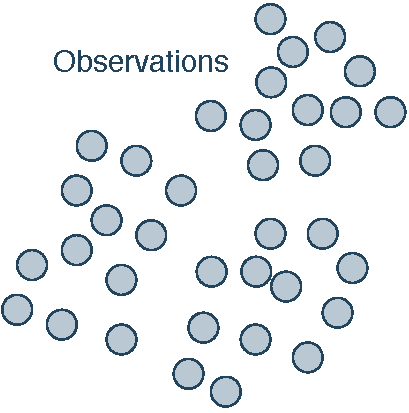
\includegraphics[scale=0.48,width=\textwidth]{figures/clusters-unassigned}
    \caption{Observations without labels. The goal is to place
      similar data points into the same clusters.}\label{fig:clusters-unassigned}
  \end{minipage}
  \hspace{5pt}
  \begin{minipage}{.46\textwidth}
    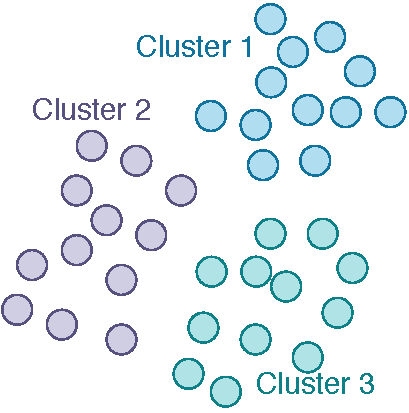
\includegraphics[scale=0.5,width=\textwidth]{figures/clusters-assigned}
    \caption{The observations have been clustered based on distance
      into three distinct clusters.}\label{fig:clusters-assigned}
  \end{minipage}
\end{figure}

\section{Motion Pattern Learning}
Motion pattern learning is the problem of learning motion patterns from a
set of trajectories, such that each pattern captures a different
characteristic of the trajectories. An example with synthetic data can be
seen in Figure~\ref{fig:motion-pattern-example}. The term
\textit{trajectory learning} is often used in the literature for the
same problem. However, in the
context of this thesis the term ``trajectory'' refers to data with
certain structure, as described in Section~\ref{sec:trajectory-data}, so 
the name motion pattern learning will be used instead.
\begin{figure}[H]
  \centering
  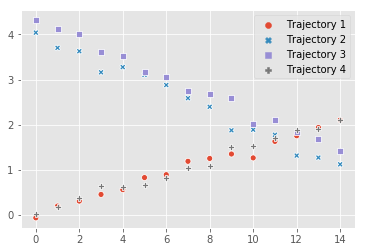
\includegraphics[width=0.7\textwidth]{figures/motion-pattern-example}
  \caption{Synthetic data showing two motion patterns with two trajectories in
    each. Trajectory 2 and 3 belong to one motion pattern and
    Trajectory 1 and 4 belong to a second motion pattern.}\label{fig:motion-pattern-example}
\end{figure}
Motion pattern learning has a natural interpretation as a
clustering problem, but clustering trajectories is difficult,
since it is hard to define a similarity metric for trajectories for
reasons described in Section~\ref{sec:trajectory-data}.

\section{Gaussian Processes}
A GP generalises a multivariate normal distribution, and can be seen
as a distribution over functions, completely defined by its
mean function $m(x)$ and covariance function $k(x, x', \hyperparam)$~\cite{Rasmussen-Williams-2006}. 
Here, $x$ and $x'$ are
elements in the domain of modeled functions, and $\hyperparam$ a
vector of hyper-parameters for the covariance function. For any input
vector $x$, the output $y$ is assumed jointly normally distributed according to
\begin{equation}
  \label{eq:gp}
  y = f(x) \sim \mathcal{N}(\mu(x), \Sigma(x))
\end{equation}
where
\begin{equation}
  \label{eq:gp-mean-function}
  \mu(x) = m(x) + K(x, \textbf{x})\textbf{V}^{-1}{(y-m(x))}^{T},
\end{equation}
\begin{equation}
  \label{eq:gp-covariance-function}
  \Sigma(x) = K(x, x) + \sigma^{2}_n\textbf{I} - \textbf{K}(x, \textbf{x})\textbf{V}^{-1}{\textbf{K}(x, \textbf{x})}^{T},
\end{equation}
and $\textbf{K}$ is the gram matrix with elements $K_{ij} = k(x_i, x_j)$ and $\textbf{V}
= K(x, x) + \sigma_n^2I$.
In the context of this thesis, the mean function $m(x)$ can be assumed to be $m(x) = 0$
without loss of generality, making the covariance function $k(x, x', \hyperparam)$
the only free parameter. Picking a specific function represents a prior
belief on how values close in $y$ are related, expressed in $x$. This
concept is explored in more detail in Section~\ref{sec:kernels-as-priors}.
Training a GP is typically done using maximum likelihood
estimation. That is, the GP parameters $\hyperparam$ are optimised to
maximise the data likelihood. Unfortunately, this is non-convex
optimisation problem, so
iterative methods have to be used. The likelihood function is
non-convex, which introduces a high risk of finding local minimas
during the optimisation process. Because of this, random restarts are
typically required to find a good $\hyperparam$.

\subsection{Kernels as Covariance Functions}\label{sec:kernels-as-priors}
Covariance function formalises a prior belief on the shape of the target
function, by specifying how correlated function values $y$ are by
evaluation the kernel function pair-wise on the observarions. 
While in practice any binary function can be plugged into
a GP, a class of functions known as \textit{kernels} are typically
used, since they have useful properties for expressing covariance. In
particular, kernels are positive-definite functions, which in turn
gives a positive-definite covariance matrix. This is required for it
to be invertable, which in turn is required to compute the GP posterior. 
The requirement of positive-definiteness makes intuitive sense, since covariance can not
be negative. 

Kernels are increadibly flexible, and can be defined for other entities than continuous
funtions, such as graphs, strings and
images~\cite{duvenaud2013structure}. However, for this thesis project
only kernels on continuous functions are considered. Kernels on
continuous functions are able to express a wide range of prior beliefs, from linearity to symmetry and
periodicity. Figure~\ref{fig:kernel-priors} illustrates several kernels
found in the literature on continuous functions together with samples from their priors.
\begin{figure}
  \centering
  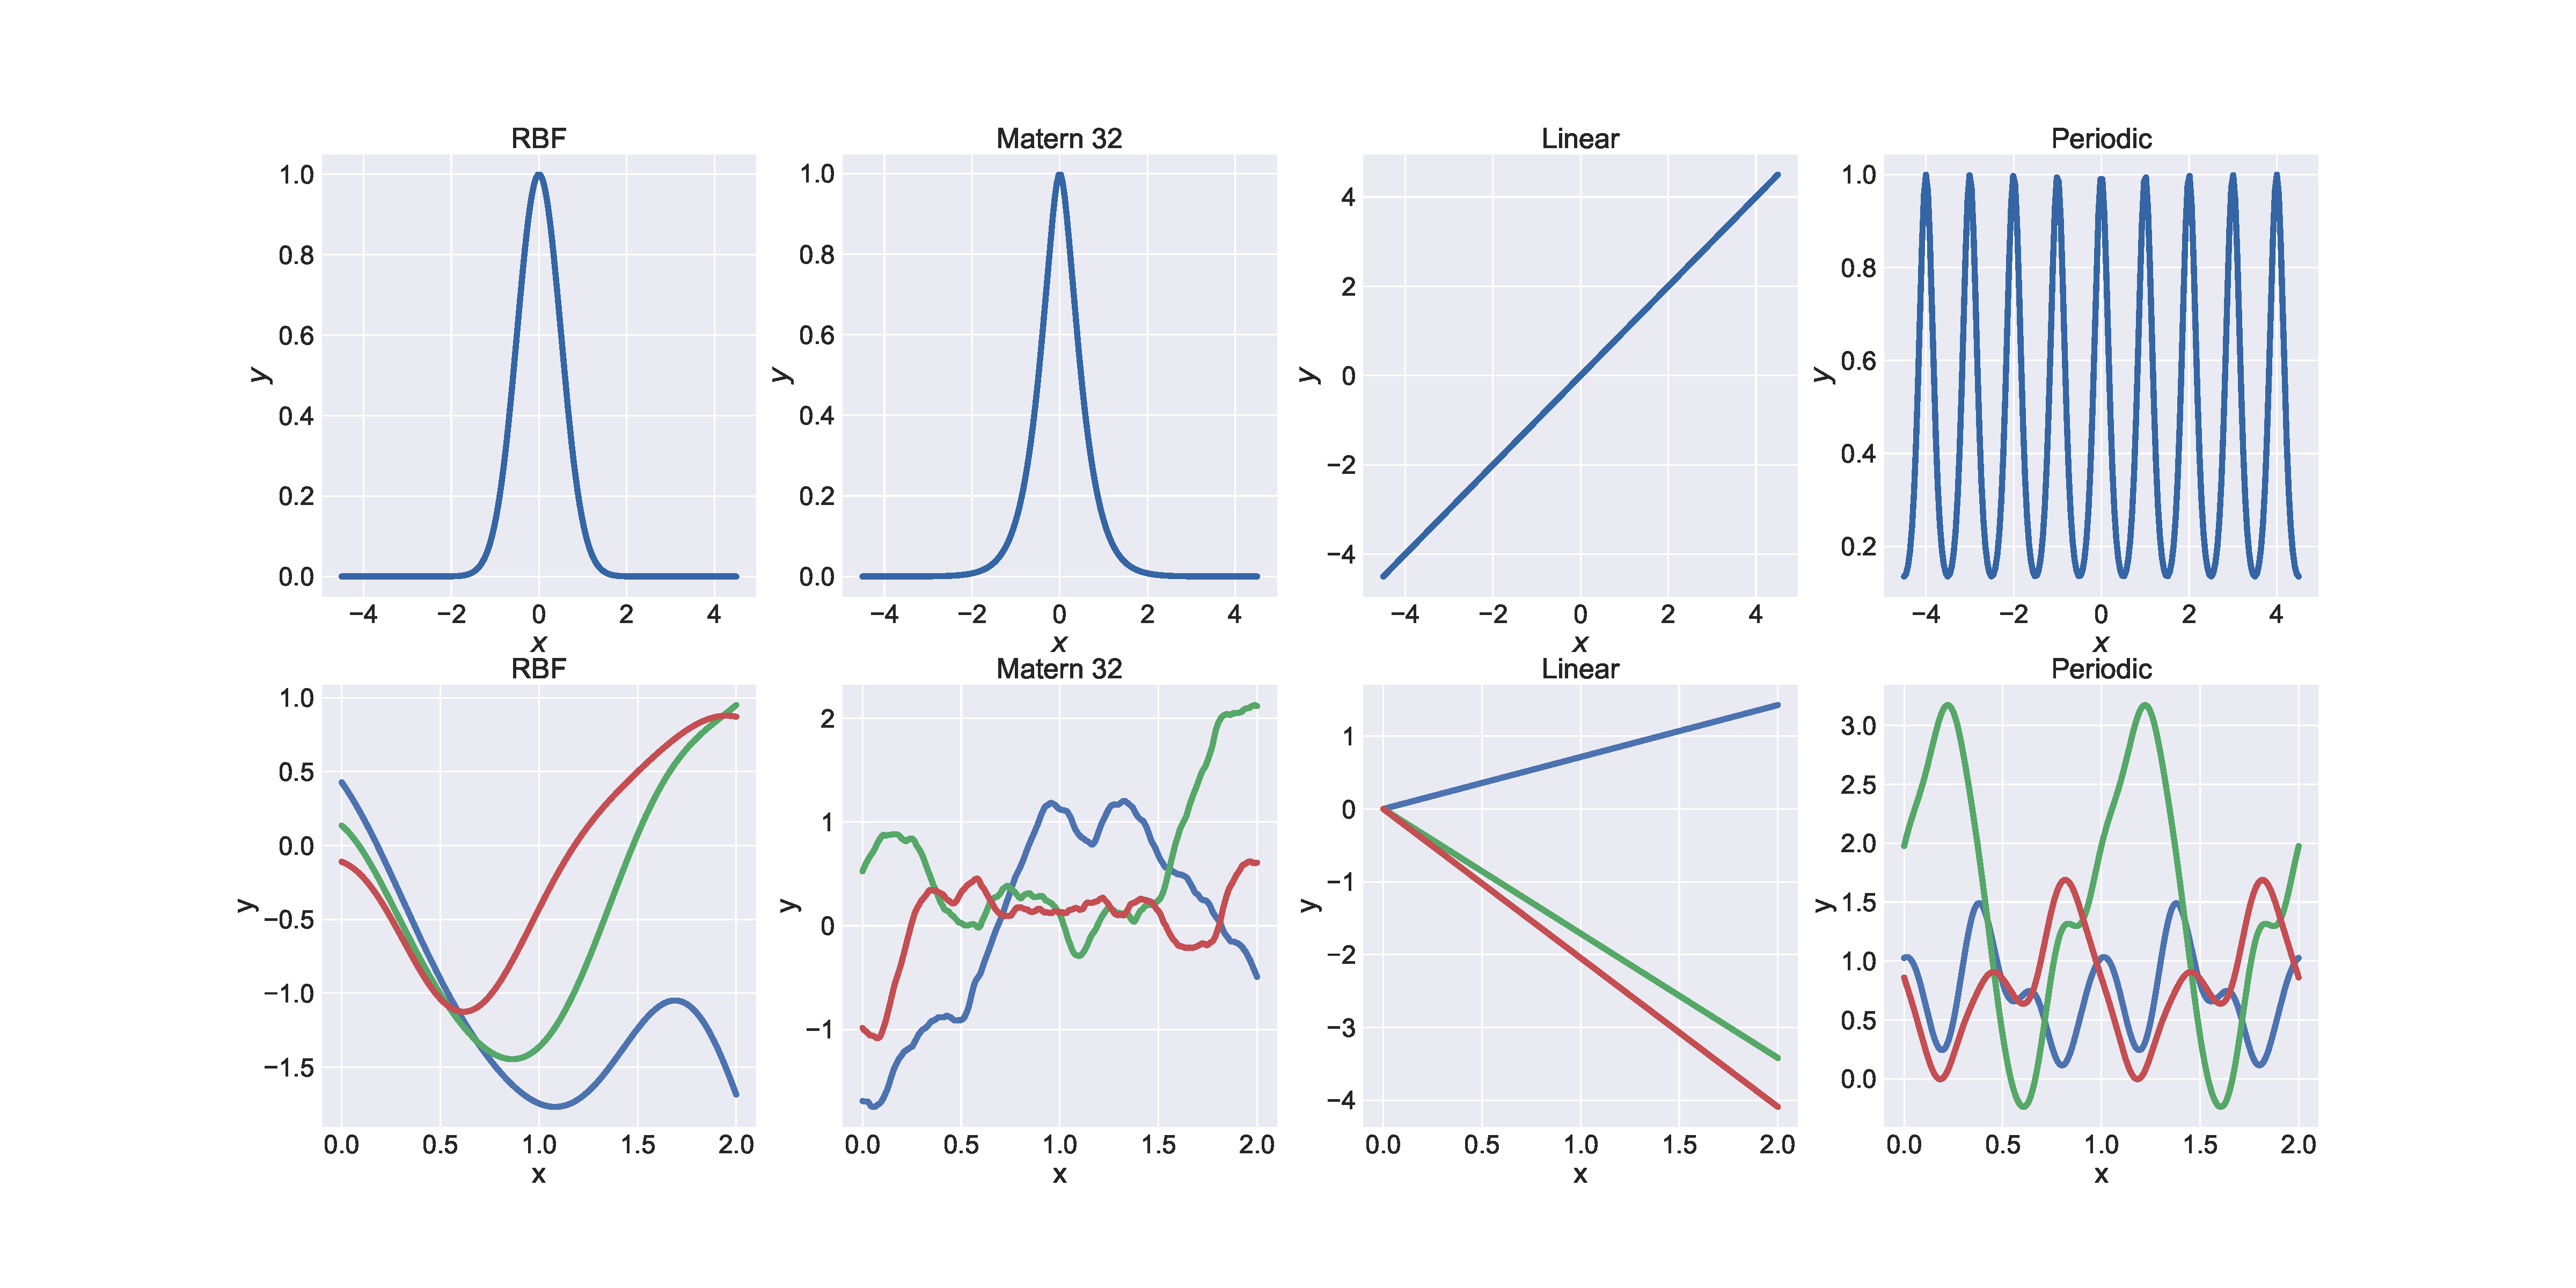
\includegraphics[width=\textwidth]{figures/kernel-priors-vert}
  \caption{Illustration of different kernels and samples from their
    priors. From left to right the kernel functions are RBF (Radial
    Basis Fuction), Matern 32, linear kernel, and periodic kernel.}\label{fig:kernel-priors}
\end{figure}

Even though a single kernel captures a lot of priors, it is sometimes
desireable to express more complicated one. Fortunately,
the set of kernel functions are closed under multiplication and addition, which
creates a principled way of combining them, creating \textit{compound
  kernels}~\cite{duvenaud2013structure}. Kernels can be combined as
required to capture prior beliefs about periodicity \textit{and}
linearity, for instance. Figure~\ref{fig:compound-kernels} illustrates
the concept of compound kernels.
\begin{figure}
  \centering
  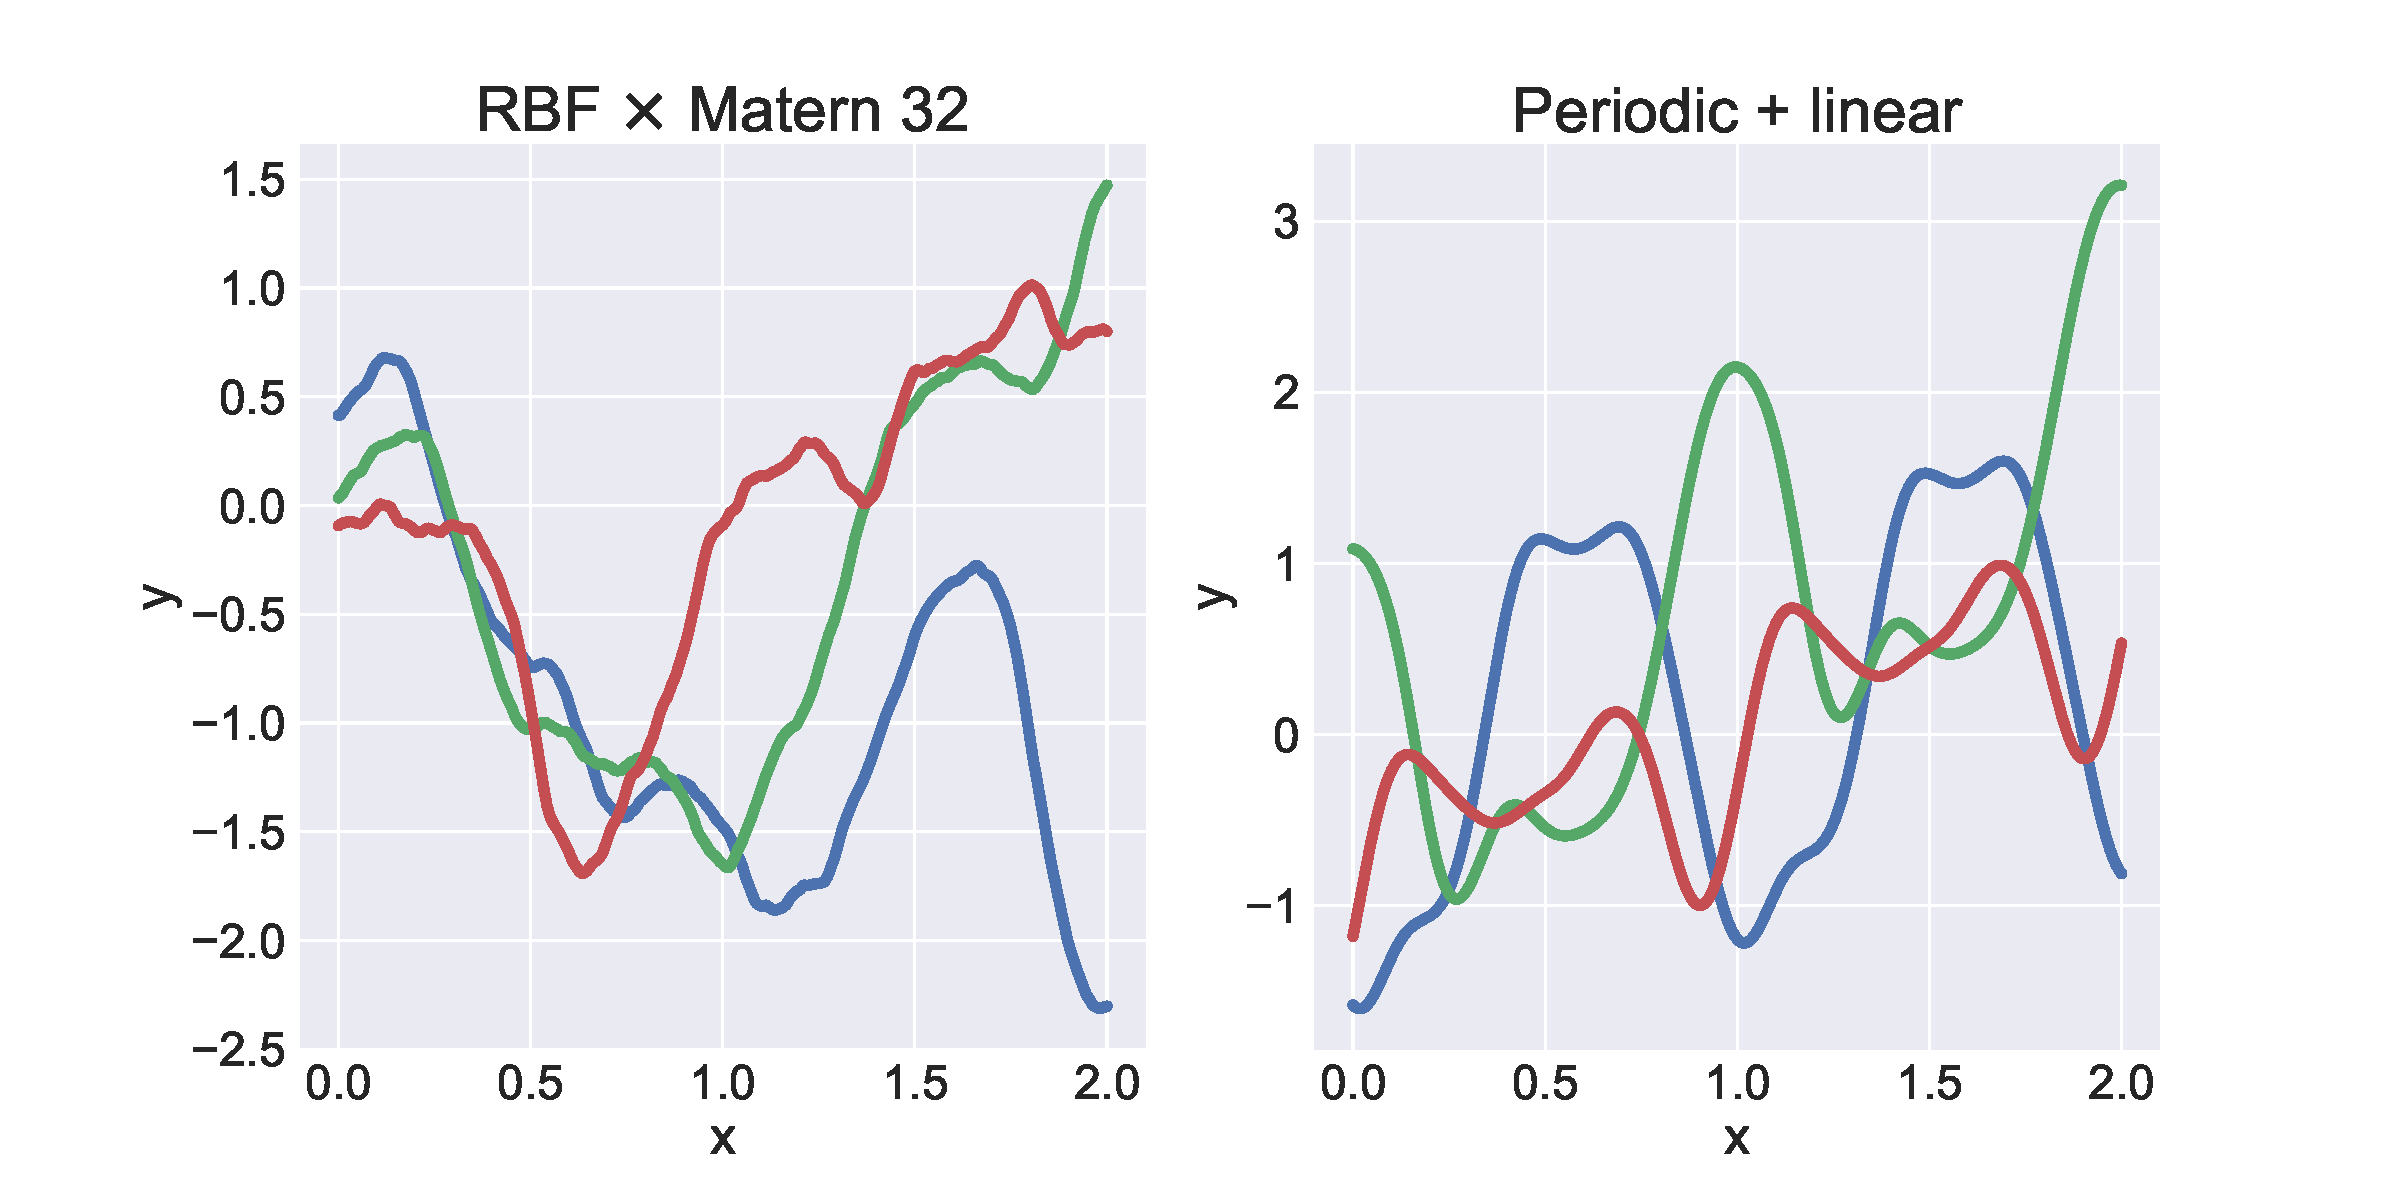
\includegraphics[width=0.75\textwidth]{figures/compound-kernels}
  \caption{Illustration of compound kernels. In the top row RBF
    and Matern 32 are combined by multiplication, and in the bottom
    row a linear and periodic kernel are combined by addition.}\label{fig:compound-kernels}
\end{figure}

\subsection{Structure Discovery Using Gaussian Processes}
Structure discovery is the problem of automatically learning the
structure of data. By creating kernels for specific characteristics
and combining them in a way that maximises the marginal likelihood, it
is possible to detect said characteristics, based on the combination
of kernels~\cite{duvenaud2013structure}.

There are infintely many ways to construct compound kernels, and some
kernel combinations explain a specific data set $X$ better than
other. How well a kernel $k$ explains $X$ can be approximated
by the Bayesian information criterion (BIC)
\begin{equation}
  BIC(k) = \log p(X \vert k) - \frac{1}{2} \vert k \vert \log N,
\end{equation}
where $\vert k \vert$ denotes the number of kernel parameters and $N$
the number of observations. BIC assumes independence between
observations conditioned on parameters, but this is in general not the
case in a GP model. However, it has been shown to be a good enough approximation~\cite{duvenaud2013structure}.
\begin{figure}
  \centering
  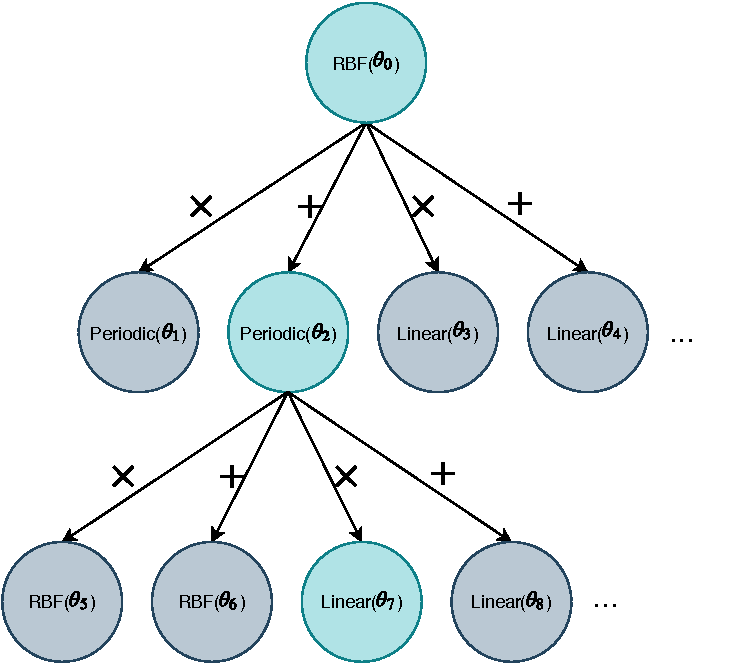
\includegraphics[width=0.75\textwidth]{figures/compound-kernel-search}
  \caption{Illustration of greedy search over kernel structures under
    multiplication and addition, where the
    expanded nodes are highlighted. Each kernels hyperparameters
    $\hyperparam_i$ are learned from data, and the kernel that
    minimises BIC the most is selected.}\label{fig:compound-kernel-search}
\end{figure}

With a way of comparing kernels established, it is interesting to find
\textit{the best} compound kernel for $X$. That is, the kernel
composition that maximises BIC. One way to do so is to
greedily search over a set of pre-defined kernel compositions, fitting
them to data as the search goes, and composing the ones that minimise
the BIS into the compound kernel. This process is illustrated in Figure~\ref{fig:compound-kernel-search}.
The structure of the resulting kernels reveals structure in the
data. For instance, if the resulting kernel contains a RBF component and a periodic
component, the data is locally correlated, and follow a periodic
trend. This process can be used to automatically detect structure in
data, from a cleaverly crafted set of kernels that correspond to
known characteristics.

\section{The Equirectangular Map Projection}
Working with data in latitude-longitude space is tricky, since the two
dimensinos are not scaled 1:1. To make it easier to work with such
data, it can be projected onto a Euclidian space, where it can be
described using cartesian coordiantes. However, since latitude and
longitude describe points on an ellipsis, and cartesian coordiantes are
orthogonal, a perfect projection does not
exist~\cite{snyder1989album}. Because of this, several different
projections have been invented, each making a different trade-off.
One of these is the \textit{Equirectangular Projection}, which maps
latitude $\phi$ and longitude $\lambda$ onto cartesian coordinates $x$
and $y$ through
\begin{equation}
  \label{eq:equirectangular-projection}
  \begin{split}
    x = (\lambda - \lambda_0)&
    \cos \phi_0 \\
    y = (\phi - \phi_0),
  \end{split}
\end{equation}
where $\lambda_0$ and $\phi_0$ define the
central meridian and the standard parallels of the latitude-longitude
space respectively. The projection is
correct for $\phi = \phi_0$, but the further away points are from
$\phi_0$ the larger the residuals will be. The $y$- and $x$--axis of
the resulting cartesian coordinate system will be $\lambda_0$ and
$\phi_0$ respectively.
